% !TeX root = ../../Book1.tex
% 纲要标题：### 2.2 仿射和 Euclid 二次对象的分类
% 纲要位置：几何学计划纲要.md，第 164 行。
% 正文状态：初稿；尚未正式审核。

% 纲要内容开始
% 
% * 二次项、线性项与中心判据
% * 平移消去线性项及其障碍
% * 二次多项式的 Euclid 与仿射标准形
% * 退化参数、直纹及实点集
% 
% 纲要内容结束

\section{仿射和 Euclid 二次对象的分类}
\label{g1:sec:0202}

平面上的椭圆、双曲线和抛物线都由二次方程给出，但它们的差别不能只从二次项的正负号读出。例如 \(x^2+y^2=1\) 与 \(x^2+y^2=-1\) 的二次项相同，后一个方程却没有实解；\(x^2-y=0\) 中的线性项则决定了一条抛物线。要分类这些对象，必须同时处理二次项、线性项和常数项，并说明坐标变换是否需要保持长度。

\subsection{二次项、线性项与中心判据}
\label{g1:subsec:0202:01}

在 \(\mathbb R^n\) 上，每个次数不超过二的实多项式都唯一写成
\begin{equation}
	\label{g1:eq:affine-quadratic-polynomial}
	F(x)=x^{\mathsf T}Ax+2b^{\mathsf T}x+c,
	\qquad A=A^{\mathsf T}.
\end{equation}
交叉项均分给 \(a_{ij}\) 与 \(a_{ji}\)，这就确定了对称矩阵 \(A\)；在线性项前写 \(2\)，是为了使配方时的公式较简洁。当 \(A\ne0\) 时，称 \(F=0\) 为一个\term[fangsheerciqumian]{仿射二次曲面}[affine quadric]的方程。这里“曲面”泛指任意维数的二次对象；在仿射平面中也称为二次曲线。

\ProseParagraphBreak

本节把方程本身保留下来：两个方程在允许的坐标变换下等价，是指相应多项式经过该变换后相差一个非零常数倍。仅把实解看成点集会丢掉信息。例如 \(x^2+y^2+1=0\) 与 \(x^2+1=0\) 都给出空集，但二次项的秩不同，不能经可逆仿射变换互相转化。为看清常数倍究竟消去了什么，我们先分类固定的多项式，再把整体非零倍数也纳入等价关系。

\begin{definition}[二次多项式的中心]
	\label{g1:def:quadric-center}
	对次数不超过二的实多项式 \(F\colon\mathbb R^n\rightarrow\mathbb R\)，若点 \(a\) 满足
	\[
		F(a+y)=F(a-y)\qquad(y\in\mathbb R^n),
	\]
	则称 \(a\) 为 \(F\) 的\term[erciduoxiangshizhongxin]{中心}[center of a quadratic polynomial]。中心存在时称该多项式有中心。
\end{definition}

这个条件使每条等值集都关于 \(a\) 中心对称，因而当然使零点集中心对称。反过来，仅检查某一个点集的对称性未必能恢复多项式条件：空集关于每一点都对称，而 \(x^2+y^2+1\) 作为多项式只有原点这个中心。

\begin{proposition}[中心判据]
	\label{g1:prop:quadric-center}
	设 \(n\) 为非负整数，\(A\) 为实对称 \(n\) 阶矩阵，\(b,a\in\mathbb R^n\)、\(c\in\mathbb R\)，并将实多项式 \(F(x)=x^{\mathsf T}Ax+2b^{\mathsf T}x+c\) 写成式\eqref{g1:eq:affine-quadratic-polynomial}的形式。点 \(a\) 是 \(F\) 的中心，当且仅当
	\[
		Aa=-b.
	\]
	中心存在当且仅当 \(b\in\operatorname{im}A\)，等价地，\(b\) 与 \(\ker A\) 正交。若 \(a_0\) 是一个中心，则全部中心构成仿射子空间 \(a_0+\ker A\)，并且 \(F\) 在这个子空间上取同一个值。
\end{proposition}

\begin{proof}
	平移原点后直接展开，得到
	\begin{equation}
		\label{g1:eq:quadratic-translation}
		F(a+y)=y^{\mathsf T}Ay+2(Aa+b)^{\mathsf T}y+F(a).
	\end{equation}
	把 \(y\) 换成 \(-y\)，两式相减为 \(4(Aa+b)^{\mathsf T}y\)。它对所有 \(y\) 为零，当且仅当 \(Aa+b=0\)。这个线性方程有解恰好意味着 \(-b\in\operatorname{im}A\)，且有解时全部解为 \(a_0+\ker A\)。

	还需说明正交条件。因为 \(A\) 对称，若 \(v\in\ker A\)，则 \(\langle Ax,v\rangle=\langle x,Av\rangle=0\)。所以 \(\operatorname{im}A\subseteq(\ker A)^\perp\)；两边维数都是 \(n-\dim\ker A\)，故相等。最后在式\eqref{g1:eq:quadratic-translation}中取中心 \(a_0\) 和 \(y\in\ker A\)，二次项、线性项都为零，得到 \(F(a_0+y)=F(a_0)\)。
\end{proof}

\begin{example}[唯一中心、一族中心与没有中心]
	\label{g1:exm:quadric-centers}
	\(F(x,y)=(x-1)^2+4(y+2)^2-1\) 的矩阵 \(A\) 可逆，中心唯一，为 \((1,-2)\)。在 \(\mathbb R^3\) 中，\(G(x,y,z)=(x-1)^2+y^2-1\) 的中心是直线 \(\{(1,0,z):z\in\mathbb R\}\)，因为沿 \(z\) 方向平移不改变多项式。对 \(H(x,y)=x^2-y\)，有 \(\ker A=\mathbb R(0,1)\)，而线性项在这个方向上不为零，所以没有中心。抛物线的顶点存在，却不是中心；顶点的作用不能由“把原点移到那里就消去全部线性项”来解释。
\end{example}

\subsection{平移消去线性项及其障碍}
\label{g1:subsec:0202:02}

平移只能消去落在二次项像空间中的线性项；剩余分量由核记录。记
\[
	\mathbb R^n=\operatorname{im}A\oplus\ker A,
	\qquad b=b_1+b_0,
	\quad b_1\in\operatorname{im}A,\quad b_0\in\ker A.
\]
这里用的是通常点积下的正交分解；它的存在与唯一性由\cref{g1:prop:projection}保证。限制 \(A|_{\operatorname{im}A}\) 是可逆的：若像空间中的向量也落在核中，它同时属于两个正交子空间，便只能为零；有限维下单射即满射。因此存在唯一 \(a\in\operatorname{im}A\) 满足 \(Aa=-b_1\)。由式\eqref{g1:eq:quadratic-translation}，
\begin{equation}
	\label{g1:eq:residual-linear-term}
	F(a+y)=y^{\mathsf T}Ay+2b_0^{\mathsf T}y+\kappa,
	\qquad \kappa=F(a).
\end{equation}
平移对 \(b\) 的影响只是加上 \(Aa\)，始终属于 \(\operatorname{im}A\)。所以投影到 \(\ker A\) 的分量 \(b_0\) 是任何平移都无法改变的障碍。

\ProseParagraphBreak

若 \(b_0=0\)，我们已经到达中心，常数 \(\kappa\) 是中心上的值。若 \(b_0\ne0\)，令 \(\beta=\lVert b_0\rVert>0\)，在核中选第一条单位坐标轴为 \(b_0/\beta\)。沿这条轴的坐标记为 \(z_1\)，剩余线性项就是 \(2\beta z_1\)。再把 \(z_1\) 平移 \(-\kappa/(2\beta)\)，就能消去常数。这个方向没有二次项，因此此次平移不会重新制造线性项或交叉项。这正是有中心与无中心两类标准形不同的原因。

\begin{example}[一次完整配方]
	\label{g1:exm:parabolic-completion}
	考虑
	\[
		F(x,y,z)=x^2+2xy+y^2+2x+2y-4z+3.
	\]
	先取正交坐标 \(u=(x+y)/\sqrt2\)、\(v=(x-y)/\sqrt2\)、\(w=z\)，得到
	\[
		F=2u^2+2\sqrt2\,u-4w+3
		=2(u+1/\sqrt2)^2-4w+2.
	\]
	令 \(U=u+1/\sqrt2\)、\(W=w-1/2\)，则方程为 \(U^2=2W\)，而 \(v\) 完全自由。它是一条抛物线沿 \(v\) 方向平移得到的柱面。这里二次项的核由 \(v,w\) 两个方向张成，但只有 \(w\) 方向上的线性项不能消去；“有核”与“没有中心”不是同一句话。
\end{example}

\subsection{二次多项式的 Euclid 与仿射标准形}
\label{g1:subsec:0202:03}

上一章已经分别给出两种对角化。\cref{g1:thm:spectral}在实有限维内积空间中用标准正交特征基消去交叉项，保留特征值；\cref{g1:thm:inertia}允许各方向分别缩放，把非零系数归一为 \(1\) 或 \(-1\)，保留正、负和零的个数。现在加上刚才的平移，就得到完整的非齐次标准形。

\begin{theorem}[二次多项式的 Euclid 标准形]
	\label{g1:thm:euclidean-quadric-normal}
	设 \(F(x)=x^{\mathsf T}Ax+2b^{\mathsf T}x+c\) 是 \(\mathbb R^n\) 上次数不超过二的实多项式，\(A\) 对称，秩为 \(k\)。通过 Euclid 坐标变换 \(x=Qy+a\)，其中 \(Q^{\mathsf T}Q=I\)，它可化为下列标准形，且恰属于其中一类：
	\begin{enumerate}
		\item 有中心时，
		\[
			F=\lambda_1y_1^2+\cdots+\lambda_ky_k^2+\kappa,
			\qquad \lambda_i\ne0,
		\]
		其余 \(n-k\) 个变量不出现。
		\item 没有中心时，\(k<n\)，且
		\[
			F=\lambda_1y_1^2+\cdots+\lambda_ky_k^2+2\beta z_1,
			\qquad \lambda_i\ne0,\quad\beta>0,
		\]
		其中 \(z_1\) 是核中的一个坐标，其余 \(n-k-1\) 个变量不出现。
	\end{enumerate}
	在第一类中，非零特征值多重集 \(\{\lambda_i\}\) 和中心值 \(\kappa\) 是完全不变量；在第二类中，完全不变量是同一个特征值多重集及 \(\beta=\lVert P_{\ker A}b\rVert\)。这里完全不变量的意思是：固定 \(n\) 后，两个多项式能由 Euclid 坐标变换相互转化，当且仅当所属类别和相应数据相同。
\end{theorem}

\begin{proof}
	由\cref{g1:cor:orthogonal-diagonalization}，可以在 \(\operatorname{im}A\) 中选择对应全部非零特征值的标准正交基，并在 \(\ker A\) 中选择标准正交基。配合式\eqref{g1:eq:residual-linear-term}及其后的核内平移，得到两种所列标准形。若 \(b_0\ne0\)，核非零，所以 \(k<n\)。这证明存在性。

	对于唯一性，任意 Euclid 坐标变换使二次项矩阵变成 \(Q^{\mathsf T}AQ\)，故特征值多重集不变。中心存在与否由定义保持，且有中心时多项式在中心上的值不变。无中心时，平移把 \(b\) 改为 \(b+Aa\)，不改变它在核中的投影；正交换基把核及这个投影同时作等距变换，故投影的长度 \(\beta\) 不变。反过来，若这些数据相同，重排非零特征轴后，两个多项式具有完全相同的标准表达式；把各自的坐标变换复合，就得到它们之间的 Euclid 变换。
\end{proof}

若分类的是方程 \(F=0\)，则还允许把 \(F\) 整体乘以 \(\mu\ne0\)。在有中心的情形，数据变成 \((\{\mu\lambda_i\},\mu\kappa)\)；在无中心的情形，数据变成 \((\{\mu\lambda_i\},|\mu|\beta)\)。这是 Euclid 方程分类中唯一需要再作的认同，不能任意改变每一个 \(\lambda_i\) 的大小。例如椭圆 \(x^2/a^2+y^2/b^2=1\) 的半轴长仍被 Euclid 等价保留。

\begin{theorem}[二次多项式的仿射标准形]
	\label{g1:thm:affine-quadric-normal}
	设 \(n\) 为非负整数，\(A\) 为实对称 \(n\) 阶矩阵，\(b\in\mathbb R^n\)、\(c\in\mathbb R\)，\(F\colon\mathbb R^n\rightarrow\mathbb R\) 为式\eqref{g1:eq:affine-quadratic-polynomial}所示的多项式 \(F(x)=x^{\mathsf T}Ax+2b^{\mathsf T}x+c\)，\(A\) 的惯性为 \((p,q,r)\)，其中 \(p+q+r=n\)。允许任意可逆仿射坐标变换后，有如下标准形与唯一性。
	\begin{enumerate}
		\item 有中心时，
		\[
			F=u_1^2+\cdots+u_p^2-v_1^2-\cdots-v_q^2+\kappa,
		\]
		其余 \(r\) 个变量不出现；\((p,q,r,\kappa)\) 是完全不变量。
		\item 没有中心时，\(r\ge1\)，且
		\[
			F=u_1^2+\cdots+u_p^2-v_1^2-\cdots-v_q^2+2z_1,
		\]
		其余 \(r-1\) 个变量不出现；\((p,q,r)\) 是完全不变量。
	\end{enumerate}
	若进一步只分类方程的非零常数倍，则第一类可写为
	\begin{equation}
		\label{g1:eq:affine-centered-quadric}
		u_1^2+\cdots+u_p^2-v_1^2-\cdots-v_q^2=\varepsilon,
		\qquad\varepsilon\in\{-1,0,1\},
	\end{equation}
	唯一的重复是 \((p,q,\varepsilon)\) 与 \((q,p,-\varepsilon)\)；第二类可写为
	\begin{equation}
		\label{g1:eq:affine-parabolic-quadric}
		u_1^2+\cdots+u_p^2-v_1^2-\cdots-v_q^2=2z_1,
	\end{equation}
	唯一的重复是交换 \(p,q\)。各式中的自由变量数仍由 \(n\) 决定。
\end{theorem}

\begin{proof}
	从 Euclid 标准形出发，对每个非零特征方向用 \(u_i=\sqrt{|\lambda_i|}\,y_i\) 缩放，即可把二次项化成正负平方和。这是\cref{g1:thm:inertia}中的同一个缩放。无中心时再用 \(z'_1=\beta z_1\)，便把线性项系数化为 \(2\)。所有缩放因相应系数非零而可逆。

	一般坐标变换 \(x=Cy+a\) 使二次项矩阵变成 \(C^{\mathsf T}AC\)。惯性定理说明 \((p,q,r)\) 不变。中心性质与中心值都由多项式本身的等式定义，也不因坐标改变而变。故所列数据是必要条件；数据相同则标准表达式相同，逆用坐标变换即得充分性。

	最后考虑方程的倍数。有中心时，若 \(\kappa\ne0\)，先乘以正数 \(1/|\kappa|\)，再缩放二次项各坐标，便得到右端 \(\varepsilon=-\operatorname{sign}\kappa\)；若 \(\kappa=0\)，右端已为零。正倍数不改变惯性，负倍数同时交换 \(p,q\) 并改变 \(\varepsilon\) 的符号，所以恰有陈述中的认同。没有中心时，常数已经消去，任意非零倍数都可由重新缩放线性坐标及二次坐标吸收；负倍数只额外交换正、负方向。固定多项式的唯一性说明不存在其他认同。
\end{proof}

上述结论也覆盖 \(A=0\) 的边界：非零线性多项式都没有中心，经仿射变换成为 \(2z_1\)；常数多项式有每一点作为中心，值 \(\kappa\) 保持不变。它们的零点集分别为超平面、空集或整个空间，但不属于本节要求 \(A\ne0\) 的二次曲面。

\begin{example}[同一仿射类中的不同 Euclid 形状]
	\label{g1:exm:ellipses-affine-euclidean}
	方程 \(x^2+4y^2=1\) 在替换 \(u=x\)、\(v=2y\) 后成为单位圆，因此与圆仿射等价。若它与单位圆 Euclid 等价，则有中心方程的分类数据应满足
	\[
		(\{1,4\},-1)=(\{\mu,\mu\},-\mu)
	\]
	至多相差特征值的次序。常数项迫使 \(\mu=1\)，而特征值不相同，矛盾。两种分类中允许的变换不同，留下的几何信息也不同。
\end{example}

\subsection{退化参数、直纹及实点集}
\label{g1:subsec:0202:04}

标准形可以直接给出实点是否存在、哪些方向完全自由，以及直线能否落在曲面中的判据。对式\eqref{g1:eq:affine-centered-quadric}，只看出现的 \(p+q\) 个变量；每一个解都可以再带上任意 \(r\) 个自由坐标。\cref{g1:tab:affine-real-quadric-types}列出实点的区别，其中假定 \(p+q>0\)。

\begin{table}[htbp]
	\centering
	\caption{有中心标准形的实点集}
	\label{g1:tab:affine-real-quadric-types}
	\begin{tabularx}{\linewidth}{@{}l l X@{}}
		\toprule
		二次项 & 右端 & 出现变量中的实解 \\
		\midrule
		\(p>0,\ q=0\) & \(\varepsilon=1\) & 单位球面；\(p=1\) 时为两点 \\
		\(p>0,\ q=0\) & \(\varepsilon=0\) & 仅原点 \\
		\(p>0,\ q=0\) & \(\varepsilon=-1\) & 空集 \\
		\(p,q>0\) & 任意 \(\varepsilon\) & 均非空；\(\varepsilon=0\) 时为过原点的二次锥 \\
		\bottomrule
	\end{tabularx}
\end{table}

半负定的情形把方程乘以 \(-1\) 即归入前三行。表中前三行来自平方和非负，最后一行则可分别用一个正方向和一个负方向取得任意实数。右端为零时，若 \(x\) 是解，则 \(tx\) 对任意实数 \(t\) 都是解，因而出现直线。右端不为零时仍可能有直线，但它们通常不经过中心。

\begin{proposition}[曲面中的仿射直线]
	\label{g1:prop:affine-quadric-line}
	设 \(A\) 为实对称 \(n\) 阶矩阵，\(b,a,v\in\mathbb R^n\)、\(c\in\mathbb R\)，且 \(v\ne0\)，并令 \(F(x)=x^{\mathsf T}Ax+2b^{\mathsf T}x+c\)。整条直线 \(a+\mathbb Rv\) 包含在 \(F=0\) 中，当且仅当
	\[
		F(a)=0,\qquad (Aa+b)^{\mathsf T}v=0,
		\qquad v^{\mathsf T}Av=0.
	\]
\end{proposition}

\begin{proof}
	把直线参数代入方程：
	\[
		F(a+tv)=F(a)+2t(Aa+b)^{\mathsf T}v+t^2v^{\mathsf T}Av.
	\]
	一元二次多项式对全部实数 \(t\) 为零，当且仅当三个系数都为零。这给出两方向的蕴含。
\end{proof}

\begin{example}[两种抛物面的直线]
	\label{g1:exm:paraboloid-lines}
	在 \(z=x^2+y^2\) 上，直线方向 \((a,b,c)\) 必须满足 \(a^2+b^2=0\)，故 \(a=b=0\)；一次项条件再迫使 \(c=0\)，与方向非零矛盾，所以曲面不包含实直线。相反，\(z=xy\) 对每个固定的 \(s\) 都包含直线
	\[
		(x,y,z)=(s,t,st)\qquad(t\in\mathbb R),
	\]
	也对每个固定的 \(t\) 包含 \((s,t,st)\) 随 \(s\) 变化的直线。这两个已给出的直线族中，各恰有一条直线通过每个曲面点。由连续变化的一族直线扫出的曲面称为\term[zhiwenqumian]{直纹曲面}[ruled surface]；这两族直线称为两个\term[zhiwenzu]{直纹族}[rulings]。\cref{g1:fig:quadric-rulings}画出其中有限段，下一节将补全这两个族，并证明它们包含该曲面射影化后的全部直线。
\end{example}

\begin{figure}[htbp]
	\centering
	% !TeX root = ../Book1.tex
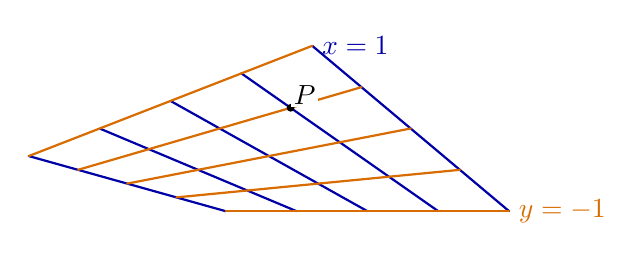
\begin{tikzpicture}[x={(1.8cm,0.35cm)},y={(-1.25cm,0.7cm)},z={(0cm,0.35cm)},line cap=round]
	\foreach \s in {-1,-0.5,0,0.5,1}{
		\draw[blue!65!black,thick] (\s,-1,{-\s}) -- (\s,1,\s);
	}
	\foreach \t in {-1,-0.5,0,0.5,1}{
		\draw[orange!85!black,thick] (-1,\t,{-\t}) -- (1,\t,\t);
	}
	\fill[black] (0.5,0.5,0.25) circle (1.4pt);
	\node[above right,fill=white,inner sep=1pt] at (0.5,0.5,0.25) {\(P\)};
	\node[blue!65!black,right] at (1,1,1) {\(x=1\)};
	\node[orange!85!black,right] at (1,-1,-1) {\(y=-1\)};
\end{tikzpicture}

	\caption[双曲抛物面的两个直纹族]{双曲抛物面 \(z=xy\) 的两个直纹族。蓝线固定 \(x\)，橙线固定 \(y\)，标出的点为 \(P=(1/2,1/2,1/4)\)。图中只画 \(-1\le x,y\le1\) 的部分，空间位置采用平行投影示意。两族线在曲面上相交，同族线互不相交。}
	\label{g1:fig:quadric-rulings}
\end{figure}

无中心标准形\eqref{g1:eq:affine-parabolic-quadric}可直接解出 \(z_1\)，因此总有实点，且是其他 \(n-1\) 个变量的图像；未出现的变量给出柱面的自由方向。有中心标准形中的自由变量也给出这种方向。例如 \(x^2+y^2=1\) 在 \(\mathbb R^3\) 中是一张圆柱面，虽然它的二次项矩阵有核，但其每一个实点附近都保持通常的圆柱形状。“矩阵有核”不能自动理解为实点集到处出现尖点或交叉。

\begin{example}[参数变化要看哪一项]
	\label{g1:exm:affine-quadric-degeneration}
	族 \(x^2+y^2=t\) 的二次项矩阵始终为 \(I_2\)，但当 \(t>0\)、\(t=0\)、\(t<0\) 时，实点集分别为圆、一个点、空集。改变的量是中心值 \(-t\)。另一族
	\[
		x^2+y^2-tz^2=1
	\]
	在 \(t<0\) 时为椭球面，\(t=0\) 时为圆柱面，\(t>0\) 时为单叶双曲面；后一名称对应截面圆半径 \(\sqrt{1+tz^2}\)，它对每个实数 \(z\) 都存在。这次发生变化的是二次项的秩与惯性。\cref{g1:prop:rank-inertia-continuity}说明，在连续实对称矩阵族中，秩固定时惯性局部不变；本例正是在 \(t=0\) 丢掉一个非零特征值，才从一个惯性类型走到另一个类型。
\end{example}

为了把二次项、线性项和常数项放进同一个对称矩阵，下一节引入一个齐次坐标。这会使上述两种看似不同的退化都能用一个齐次二次型描述，也会说明椭圆、抛物线和双曲线为何可能属于同一个射影类型。
